\documentclass[12pt]{revtex4-1}

\usepackage{graphicx} % needed for figures
\graphicspath{ {Figures/} }
\usepackage{epstopdf}
\usepackage[caption=false]{subfig}
\usepackage{amsmath}
\usepackage{amsfonts}
\usepackage{amssymb}
\usepackage{bm}
\usepackage{hyperref}
\usepackage{amsthm}
\usepackage{color}
\newcommand{\DB}[1]{\textcolor{cyan}{#1}}
\usepackage{mathrsfs}
\usepackage[vlined,ruled]{algorithm2e}
%\usepackage{subfigure}
%\usepackage{cite}
\usepackage{url}
\usepackage{color}
\usepackage{algorithmic}
\usepackage{bbm}
\usepackage{booktabs}
\usepackage{array}
\usepackage[table]{xcolor}
\usepackage{yfonts}

\newtheorem{theorem}{Theorem}[section]
\newtheorem{lemma}[theorem]{Lemma}
\newtheorem{definition}{Definition}
\newtheorem{corollary}[theorem]{Corollary}
\newtheorem{proposition}[theorem]{Proposition}
\newtheorem{problem}{Problem}
\newtheorem{remark}{Remark}
\newtheorem{assumption}{Assumption}
\newtheorem{example}{Example}

\newcommand{\mc}{\mathcal}
\newcommand{\Ker}{\operatorname{Ker}}
\newcommand{\Rank}{\operatorname{Rank}}
\newcommand{\Image}{\operatorname{Im}}
\newcommand{\real}{\mathbb{R}}
\newcommand{\complex}{\mathbb{C}}
\newcommand{\ora}[1]{\overrightarrow{#1}}
\newcommand{\map}[3]{#1: #2 \rightarrow #3}
\newcommand{\subscr}[2]{{#1}_{\textup{#2}}}
\newcommand{\supscr}[2]{{#1}^{\textup{#2}}}

\begin{document}
\title{Design of Mechanical Motions with Discrete Dynamical Systems}
\date{\today}
\begin{abstract}
	The function of many mechanical systems often depends on conformational changes in structure. To achieve desired functions, we must first accomplish the design of desired conformational changes. Here, we model mechanical systems as linkages of rigid bonds (edges) connected by joints (nodes), and map this design problem to the theory of discrete dynamical systems. Specifically, we begin by showing that a small linkage module can be thought of as one dimensional map of node distances. Next, we demonstrate that combining these modules together is equivalent to an iteration of this map. Finally, we demonstrate the design power of this map by constructing mechanical networks that display fixed points, limit cycles, and aperiodicity.
\end{abstract}
\maketitle

\section{Mathematical Framework}
\subsection{Mechanical Networks}
Consider a set of $N$ nodes $\mc V = \{1, \dotsm, N\}$ connected by $E$ pairwise edges $\mc E \subset \mc V \times \mc V$ in $d$-dimensional space. Each node $i$ has a real vector of coordinates $\bm{x}_i \in \real^d$, and the edge $k$ between nodes $i,j$ has squared length given by
\begin{align*}
l_k^2 = (\bm{x}_i - \bm{x}_j)^T(\bm{x}_i - \bm{x}_j).
\end{align*}
To enforce rigid edges, we take the time derivative of the length, and set $\dot{l}_k = 0$ such that
\begin{align*}
2l_k\dot{l}_k = 2(\bm{x}_i-\bm{x}_j)^T(\dot{\bm{x}}_i-\dot{\bm{x}}_j) = 0
\end{align*}
We can concatenate all node coordinates into column vector $\bm{x} = [\bm{x}_1; \dotsm; \bm{x}_N] \in \real^{dN}$, and all edge measurements into column vector $\bm{l} = [l_1^2; \dotsm; l_k^2]$. Then the coordinates yield $dN$ free variables, while the rigid edges yield $E$ constraints given by $\dot{\bm{l}} = \bm{0}$ such that we have $dN - E$ possible motions by constraint counting. Among these, $d(d+1)/2$ are rigid body translations and rotations, for $D$ conformational motions given by
\begin{align*}
D = dN - E - \frac{d(d+1)}{2}.
\end{align*}

\subsection{Dynamical Systems}
Additionally, consider a one-dimensional discrete-time dynamical system with state variable $y_n \in \real$ at some time $n \in \mathbb{Z}_{\geq 0}$ that evolves according to
\begin{align*}
y_{n+1} = f(y_n). 
\end{align*}
This iterated map exists in a $k$-cycle if
\begin{align*}
y_{n+k} = f^k(y_n),
\end{align*}
where $f^k$ implies the application of the map $k$-times. This $k$-cycle is stable if the product of slopes evaluated along the cycle $y_{n+1},\dotsm,y_{n+k}$
\begin{align*}
s = \prod_{i=1}^k \frac{d}{dy}f(y)\bigg|_{y_{n+i}},
\end{align*}
has magnitude less than $|s| < 1$. 




\section{Mechanical Modules as a Discrete-Time Map}

\begin{figure}[h!]
	\centering
	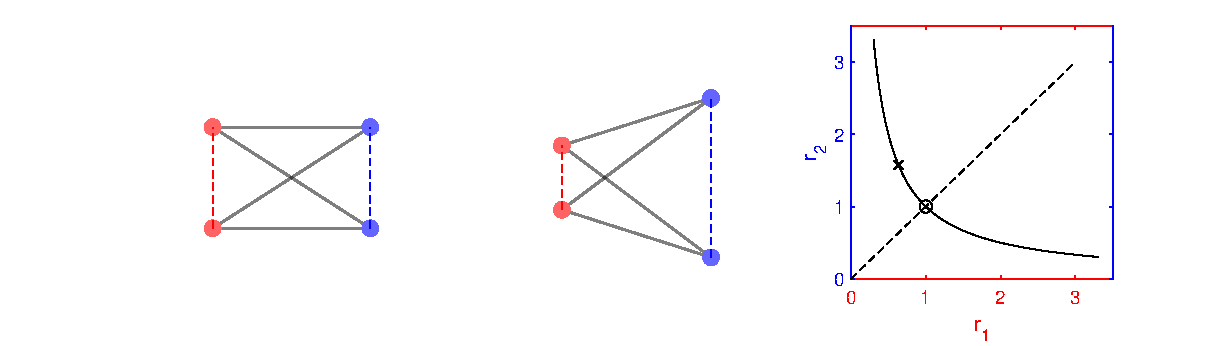
\includegraphics[width=1.0\columnwidth]{4bar.pdf}
	\caption{\textbf{Combining Network Motions by Merging Nodes and Adding Edges} (\textbf{a}) }
	\label{fig:mn_combine}
\end{figure}






\end{document}
